\documentclass[12pt, letterpaper]{article}
\usepackage[margin=1in]{geometry}
\usepackage[T1]{fontenc}
\usepackage{lmodern}
\usepackage{cmap}
\usepackage[utf8]{inputenc}
\usepackage{amsmath, amssymb, amsthm}
\usepackage{mathtools}
\usepackage{enumitem}
\usepackage{booktabs}
\usepackage{xcolor}
\usepackage{titlesec}
\usepackage{parskip}
\usepackage{hyperref}
\usepackage{fancyhdr}
\usepackage{tcolorbox}
\usepackage{graphicx}
\usepackage{caption}
\tcbuselibrary{skins, breakable}

\definecolor{darkblue}{RGB}{15,55,115}
\definecolor{midblue}{RGB}{30,100,180}
\definecolor{theorybg}{RGB}{245,250,255}
\definecolor{questionbg}{RGB}{255,252,240}
\definecolor{evencolor}{RGB}{60,0,100}

\hypersetup{colorlinks=true,linkcolor=darkblue,urlcolor=midblue,
  pdftitle={Kurlat --- A Course in Modern Macroeconomics --- Complete Solutions, Chapter 9}}

\setlength{\headheight}{14pt}
\pagestyle{fancy}
\fancyhf{}
\renewcommand{\headrulewidth}{0.4pt}
\fancyhead[L]{\small\textcolor{darkblue}{\textit{Kurlat --- A Course in Modern Macroeconomics}}}
\fancyhead[R]{\small\textcolor{darkblue}{\thepage}}
\fancyfoot[C]{\small\textcolor{gray}{Complete Solutions --- Chapter 9}}

\titleformat{\section}[block]
  {\large\bfseries\color{darkblue}}{}{0pt}{}
  [\vspace{2pt}\color{darkblue}\rule{\textwidth}{1.5pt}\vspace{4pt}]

\titleformat{\subsection}[block]
  {\normalsize\bfseries\color{midblue}}{}{0pt}{}
  [\vspace{1pt}\color{midblue}\rule{0.5\textwidth}{0.8pt}\vspace{3pt}]

\tcbset{
  theorybox/.style={
    enhanced,breakable,colback=theorybg,colframe=darkblue,
    fonttitle=\bfseries\small\color{darkblue},boxrule=0.5pt,arc=3pt,
    left=6pt,right=6pt,top=4pt,bottom=4pt,title={Key Theory},
  },
  questionbox/.style={
    enhanced,breakable,colback=questionbg,colframe=gray!60,
    fonttitle=\bfseries\small\color{gray!60!black},boxrule=0.4pt,arc=2pt,
    left=6pt,right=6pt,top=4pt,bottom=4pt,title={\textit{Question}},
  },
  oddbox/.style={
    enhanced,breakable,colback=white,colframe=darkblue,
    attach boxed title to top left={yshift=-2mm,xshift=6mm},
    boxed title style={colback=darkblue,colframe=darkblue,arc=2pt,
      boxrule=0pt,left=6pt,right=6pt,top=3pt,bottom=3pt},
    fonttitle=\bfseries\large\color{white},
    boxrule=0.8pt,arc=3pt,
    left=8pt,right=8pt,top=10pt,bottom=6pt,
  },
  evenbox/.style={
    enhanced,breakable,colback=white,colframe=evencolor,
    attach boxed title to top left={yshift=-2mm,xshift=6mm},
    boxed title style={colback=evencolor,colframe=evencolor,arc=2pt,
      boxrule=0pt,left=6pt,right=6pt,top=3pt,bottom=3pt},
    fonttitle=\bfseries\large\color{white},
    boxrule=0.8pt,arc=3pt,
    left=8pt,right=8pt,top=10pt,bottom=6pt,
  },
  databox/.style={
    enhanced,breakable,colback=gray!8,colframe=gray!55,
    fonttitle=\bfseries\small\color{gray!60!black},boxrule=0.4pt,arc=2pt,
    left=6pt,right=6pt,top=4pt,bottom=4pt,title={Numerical exercise --- see the companion code},
  },
  trapbox/.style={
    enhanced,breakable,colback=red!4,colframe=red!45!black,
    fonttitle=\bfseries\small\color{white},boxrule=0.4pt,arc=2pt,
    coltitle=white,
    left=6pt,right=6pt,top=4pt,bottom=4pt,title={Where this goes wrong},
  },
}

\newcommand{\pd}[2]{\dfrac{\partial #1}{\partial #2}}
\newcommand{\dd}[2]{\dfrac{d #1}{d #2}}
\newcommand{\MRS}{\mathrm{MRS}}
\newcommand{\MRT}{\mathrm{MRT}}
\newcommand{\MU}{\mathrm{MU}}
\newcommand{\Var}{\mathrm{Var}}
\newcommand{\Cov}{\mathrm{Cov}}
\newcommand{\E}{\mathrm{E}}
\newcommand{\MPK}{\mathrm{MPK}}
\newcommand{\MPL}{\mathrm{MPL}}
\newcommand{\stst}{^{\ast}}

\setlist[enumerate,1]{label=(\alph*),itemsep=6pt,parsep=2pt}
\setlist[enumerate,2]{label=(\roman*),itemsep=3pt}

\begin{document}

%======================================================================
% TITLE PAGE
%======================================================================
\begin{titlepage}
\centering
\vspace*{2.5cm}
{\Huge\bfseries\color{darkblue} A Course in Modern Macroeconomics\par}
\vspace{6pt}
{\large Pablo Kurlat (2020)\par}
\vspace{1.4cm}
{\LARGE\bfseries Complete Solutions\par}
\vspace{6pt}
{\LARGE\bfseries Chapter 9 --- General Equilibrium\par}
\vspace{1.2cm}
{\large All thirteen end-of-chapter problems, 9.1--9.13 (pp.~179--188)\par}
\vspace{2cm}

\begin{tcolorbox}[theorybox,title={What is in this file},width=0.86\textwidth]
\small
Every problem carries the full question text, a step-by-step solution with no skipped
algebra, an economic reading of the result, and a verification. Numerical answers are
reproduced by the companion scripts in \texttt{Resolucao/kurlat\_ch09\_codigo/}, which
check each analytical formula against an independent computation and abort on any
mismatch.

\smallskip
Problems are grouped by \textbf{topic}, not by number, following the order of the
chapter's own sections. Blue boxes are odd-numbered problems, purple boxes even.

\smallskip
This is a companion to \texttt{kurlat\_solutions\_ch1-4.tex}; chapters 5--7 are not yet
covered and chapter 8 is outside the course syllabus.
\end{tcolorbox}

\vfill
{\small MPE Insper --- Macroeconomia I --- 2026, 3\textordmasculine{} trimestre\par}
\end{titlepage}

\tableofcontents
\newpage

%======================================================================
\section{Chapter 9 \quad General Equilibrium}
%======================================================================

\begin{tcolorbox}[theorybox,title={Chapter 9 Overview}]
The chapter closes the model. Chapters 6--8 studied households and firms one at a time;
here all the decisions are held simultaneously and the prices that make them consistent
are solved for.

\smallskip
\textbf{Three agents.} A representative household choosing consumption, saving and
leisure; a representative firm renting capital and hiring labour; and a representative
\emph{investment firm} that buys used capital, adds investment, and rents the result out
next period. The third agent is the one students have not met before, and its problem
(9.1.2) is \emph{linear} in investment --- which is why its first-order condition
determines a \textbf{price}, $1+r=r^K_2$, and not a quantity.

\smallskip
\textbf{The collapse.} Combining the five first-order conditions makes every price cancel,
leaving
\[
\underbrace{\frac{v'(l_t)}{u'(c_t)}}_{\MRS}=\underbrace{F_L(K_t,L_t)}_{\MRT},
\qquad
\underbrace{\frac{u'(c_1)}{\beta u'(c_2)}}_{\MRS}=\underbrace{F_K(K_2,L_2)}_{\MRT}.
\]
\textbf{The theorem.} Proposition 9.1 shows this was no accident: a benevolent planner
constrained only by technology writes the same two equations. The theorem fails under
monopoly power, externalities, asymmetric information, incomplete markets and borrowing
constraints --- and naming which one is active is how the chapter says policy analysis
should begin.

\smallskip
\textbf{The dynamics.} With an infinite horizon, fixed labour and CRRA utility, the model
reduces to two difference equations that can be drawn as a phase diagram. The steady state
satisfies $F_K(K\stst,1)-\delta=\frac{1}{\beta}-1$, which lies strictly \emph{below} the
Golden Rule --- and that is optimal, not a failure.
\end{tcolorbox}

%---- Topic: Equilibrium Prices and Allocations ----
\subsection{Equilibrium Prices and Allocations}

%------- 9.2 -------
% Topic: Equilibrium Prices and Allocations
% Keywords: linear technology, marginal product, interest rate, Euler equation, impatience
\begin{tcolorbox}[evenbox,title={Problem 9.2 \quad Storage}]
\begin{tcolorbox}[questionbox]
Suppose the production function is the following:
\[F(K,L)=K\]
and the rate of depreciation is $\delta=1$.\\[3pt]
(a) Why is this production function called ``storage''?\\
(b) What will be the real interest rate and the wage in this economy?\\
(c) With standard preferences, will consumption increase over time, remain constant over
time or decrease over time?
\end{tcolorbox}

\textbf{Solution:}

\begin{enumerate}
\item Because the technology does nothing except carry goods forward in time. Put one unit
of the good aside as capital today and you get exactly one unit of output tomorrow. There
is no transformation, no gain and no loss --- it is a warehouse. Two features make this
literal:
\begin{itemize}
\item $F_K=1$: the marginal product of capital is one, and constant. There are
\textbf{no diminishing returns}, so the tenth unit stored is as productive as the first.
\item $F_L=0$: labour is completely useless. It does not appear in the production function.
\end{itemize}
With $\delta=1$ the stored good is consumed entirely when withdrawn, which is what
``taking it out of the warehouse'' means.

\item Read the prices straight off the firm's first-order conditions (9.1.9) and (9.1.10):
\[
r^K_t=F_K(K_t,L_t)=1,\qquad\qquad w_t=F_L(K_t,L_t)=\boxed{0}.
\]
The interest rate comes from the investment firm's arbitrage condition (9.3.11):
\[
r_{t+1}=r^K_{t+1}-\delta=1-1=\boxed{0}.
\]

\emph{Reading.} The wage is zero because labour produces nothing, and in a competitive
market a factor is paid its marginal product. The interest rate is zero because storing a
good returns exactly the good: lending one unit and getting one unit back is a zero net
return. Note that both prices are \textbf{independent of the capital stock}, which is
unusual --- with diminishing returns they would move as $K$ moved. Here the technology is
linear, so it pins the prices down once and for all.

\item Take the Euler equation (9.3.8) and substitute $r=0$:
\[
u'(c_t)=\beta(1+r)\,u'(c_{t+1})=\beta\,u'(c_{t+1}).
\]
Since the household is impatient, $\beta<1$, this gives $u'(c_t)<u'(c_{t+1})$. With
standard preferences $u'$ is strictly decreasing, so
\[
\boxed{c_t>c_{t+1}}\qquad\text{--- consumption \textbf{falls} over time.}
\]

\emph{Reading.} The technology offers a zero return on waiting, but the household strictly
prefers the present. When the market rate of return ($r=0$) falls short of the rate of time
preference ($\rho=\frac{1}{\beta}-1>0$), the household front-loads: it draws the warehouse
down, consuming more now and less later. The capital stock declines monotonically to zero.

\smallskip
\textbf{Verification.} The general condition is that consumption rises, is flat, or falls
according as $\beta(1+r)$ exceeds, equals, or falls short of one. Here
$\beta(1+r)=\beta<1$. \checkmark\ Consistent with the general steady-state condition
(9.3.17): a steady state would need $F_K-\delta=\frac{1}{\beta}-1>0$, but $F_K-\delta=0$
always, so \textbf{no steady state with positive capital exists} --- confirming that the
economy must be running down.
\end{enumerate}
\end{tcolorbox}

%------- 9.5 -------
% Topic: Equilibrium Prices and Allocations
% Keywords: linear technology, labour supply, log utility, Jones-Klenow welfare, preference heterogeneity
\begin{tcolorbox}[oddbox,title={Problem 9.5 \quad Differences in Preferences}]
\begin{tcolorbox}[questionbox]
There are two countries: Industria and Lethargia. Both have population 1 and identical
production functions $Y=AL$, where $L$ is total time spent in market labour. Preferences are
\[u(c,l)=\log(c)+\theta\log(l)\tag{9.3.18}\]
where $c$ is consumption and $l$ is leisure. Within each country everyone is identical, but
$\theta$ differs across the two: denote the values $\theta_I$ and $\theta_L$, with
$\theta_L>\theta_I$. Both countries run free-market economies with perfectly competitive
labour markets.\\[3pt]
(a) What is the wage in each country?\\
(b) Set up the problem of a representative household dividing its time (normalised to 1)
between market work and leisure.\\
(c) What fraction of its time will the household spend in market work in each country?\\
(d) Which country has higher GDP?\\
(e) Suppose a researcher (i) assumes preferences are the same everywhere, with form
(9.3.18); (ii) estimates $\theta$ using data from Lethargia; (iii) gathers consumption and
leisure data for each country; (iv) computes $\lambda$, the relative welfare of Industria,
taking Lethargia as the benchmark with $\lambda=1$, the way Jones and Klenow took the US as
benchmark. Find an expression for $\lambda$. Which country would the researcher conclude has
the higher standard of living? Explain.
\end{tcolorbox}

\textbf{Solution:}

\begin{enumerate}
\item The technology is linear in labour, so the firm's problem
$\max_L\ AL-wL=(A-w)L$ is linear too. By the same argument that pins down (9.1.11), a
positive but finite amount of labour is hired only if the coefficient is exactly zero:
\[
\boxed{w=A}\qquad\text{in \emph{both} countries.}
\]
Preferences do not enter. This is the key structural fact of the problem: the two countries
face \textbf{identical prices} and differ only in what they want.

\item With $l+L=1$ and no non-labour income, the household solves
\[
\max_{L\in[0,1]}\ \log\big(A L\big)+\theta\log(1-L).
\]

\item First-order condition:
\[
\frac{1}{L}-\frac{\theta}{1-L}=0
\;\Longrightarrow\;
1-L=\theta L
\;\Longrightarrow\;
\boxed{L\stst=\frac{1}{1+\theta}},\qquad l\stst=\frac{\theta}{1+\theta}.
\]
Note that $A$ has dropped out entirely: with log consumption utility and no non-wage income,
the income and substitution effects of the wage cancel exactly, so hours do not depend on
the wage. Since $\theta_L>\theta_I$,
\[
L_I=\frac{1}{1+\theta_I}>\frac{1}{1+\theta_L}=L_L .
\]
Industria works more. \emph{The names are not decoration.}

\item $Y_i=A L_i$, so
\[
\frac{Y_I}{Y_L}=\frac{L_I}{L_L}=\frac{1+\theta_L}{1+\theta_I}>1 .
\]
\textbf{Industria has higher GDP}, and higher consumption, since $c_i=Y_i$.

\item The researcher imposes $\theta=\theta_L$ on both countries and defines $\lambda$ by
\[
\log\big(\lambda\,c_L\big)+\theta_L\log(l_L)=\log(c_I)+\theta_L\log(l_I),
\]
that is, by how much Lethargia's consumption would have to be scaled to make a
Lethargian-preference household indifferent between the two bundles. Solving,
\[
\log\lambda=\log\frac{c_I}{c_L}+\theta_L\log\frac{l_I}{l_L}
\;\Longrightarrow\;
\boxed{\ \lambda=\frac{c_I}{c_L}\left(\frac{l_I}{l_L}\right)^{\theta_L}\ }.
\]
Substituting $c_i=A/(1+\theta_i)$ and $l_i=\theta_i/(1+\theta_i)$:
\[
\lambda=\frac{1+\theta_L}{1+\theta_I}
\left[\frac{\theta_I(1+\theta_L)}{\theta_L(1+\theta_I)}\right]^{\theta_L}.
\]

\textbf{A concrete case.} Take $\theta_I=0{,}5$ and $\theta_L=2$, with $A=1$:
\begin{center}
\begin{tabular}{lccc}
\toprule
& $L\stst$ & $c$ & $l$ \\
\midrule
Industria ($\theta_I=0{,}5$) & $0{,}667$ & $0{,}667$ & $0{,}333$ \\
Lethargia ($\theta_L=2$) & $0{,}333$ & $0{,}333$ & $0{,}667$ \\
\bottomrule
\end{tabular}
\end{center}
\[
\lambda=\frac{0{,}667}{0{,}333}\left(\frac{0{,}333}{0{,}667}\right)^{2}
=2\times 0{,}25=\boxed{0{,}5}.
\]
The researcher concludes that Industria's standard of living is \textbf{half} Lethargia's
--- despite Industria having \emph{twice} the GDP.

\smallskip
\textbf{Why, and why it is wrong.} The researcher has priced Industria's leisure using
\emph{Lethargia's} taste for it. Industria takes little leisure, and under $\theta_L$ that
shortfall is charged at a very high rate. Redo the same calculation with $\theta_I$ instead:
\[
\lambda'=\frac{c_I}{c_L}\left(\frac{l_I}{l_L}\right)^{\theta_I}
=2\times(0{,}5)^{0{,}5}=1{,}414>1,
\]
and the conclusion \textbf{reverses}. Both countries are at their own optimum given their
own preferences; neither is making a mistake, and the ranking is an artefact of whose
utility function was used.
\end{enumerate}

\begin{tcolorbox}[trapbox]
The exercise is a warning label on the Jones--Klenow welfare measure of Chapter 2. That
method is sound when preferences really are common and only \emph{opportunities} differ.
When the differences are in \emph{preferences}, the consumption-equivalent number stops
measuring welfare and starts measuring how unlike the benchmark country the other one is.
Reporting $\lambda$ without saying whose $\theta$ was used is not an incomplete answer, it
is a meaningless one.
\end{tcolorbox}
\end{tcolorbox}

%------- 9.7 -------
% Topic: Equilibrium Prices and Allocations
% Keywords: demographics, factor prices, steady state, capital-labour ratio, cohort size
\begin{tcolorbox}[oddbox,title={Problem 9.7 \quad Getting Old}]
\begin{tcolorbox}[questionbox]
An economy has two types of households: young and old. Let $\mu$ be the fraction that is
young. Total population is held constant and we consider the effects of higher or lower
$\mu$ (which could result from differences in fertility and mortality). Each young household
supplies $x$ units of labour inelastically, so total young labour is $L^Y=\mu x$; old
households supply $z$ units, also inelastically, so total old labour is $L^O=(1-\mu)z$.
Assume $x>z$. The production function is $Y=K^\alpha L^{1-\alpha}$, where $K$ is the capital
stock and $L\equiv L^Y+L^O$.\\[3pt]
(a) Holding $K$ constant, how do GDP, wages and the rental rate of capital depend on
$\mu$?\\
(b) How will the steady-state capital stock compare between two economies with different
levels of $\mu$? Explain.\\
(c) Now imagine the economy does not use capital and the production function is
$Y=(L^Y)^\gamma (L^O)^{1-\gamma}$. How do the wage levels of young and old workers depend on
$\mu$?
\end{tcolorbox}

\textbf{Solution:}

\begin{enumerate}
\item Total effective labour is
\[
L(\mu)=\mu x+(1-\mu)z=z+\mu(x-z),\qquad \dd{L}{\mu}=x-z>0 .
\]
A younger population supplies more labour, because the young work more. Holding $K$ fixed:
\begin{center}
\renewcommand{\arraystretch}{2.0}
\begin{tabular}{@{}llc@{}}
\toprule
& \textbf{Derivative with respect to $\mu$} & \\
\midrule
$Y=K^\alpha L^{1-\alpha}$
  & $\pd{Y}{\mu}=(1-\alpha)K^\alpha L^{-\alpha}(x-z)>0$ & \textbf{GDP rises} \\
$w=(1-\alpha)K^{\alpha}L^{-\alpha}$
  & $\pd{w}{\mu}=-\alpha(1-\alpha)K^\alpha L^{-\alpha-1}(x-z)<0$ & \textbf{wage falls} \\
$r^K=\alpha K^{\alpha-1}L^{1-\alpha}$
  & $\pd{r^K}{\mu}=\alpha(1-\alpha)K^{\alpha-1}L^{-\alpha}(x-z)>0$ & \textbf{rental rises} \\
\bottomrule
\end{tabular}
\end{center}
\emph{Reading.} With capital fixed, more labour means less capital per worker. Labour becomes
the abundant factor and is paid less; capital becomes the scarce one and is paid more. This
is the same comparative static as the Black Death (Exercise 4.2) run in reverse.

\item Now let capital adjust. In steady state, (9.3.17) requires
\[
F_K(K\stst,L)-\delta=\frac{1}{\beta}-1
\;\Longrightarrow\;
\alpha\left(\frac{K\stst}{L}\right)^{\alpha-1}=\frac{1}{\beta}-1+\delta .
\]
The left side depends on $K$ and $L$ \textbf{only through the ratio} $K/L$, and the right
side contains no demographic variable at all. Therefore
\[
\boxed{\ \frac{K\stst}{L}\ \text{is independent of }\mu\ }
\qquad\Longrightarrow\qquad
K\stst(\mu)=L(\mu)\left[\frac{\alpha}{\frac{1}{\beta}-1+\delta}\right]^{\frac{1}{1-\alpha}} .
\]
The younger economy has a \textbf{proportionally larger} capital stock, and exactly the same
capital per unit of labour.

\smallskip
\emph{Reading, and the contrast with (a).} Part (a) held $K$ fixed and found the wage
falling. Part (b) lets $K$ adjust and the wage
$w=(1-\alpha)(K\stst/L)^{\alpha}$ is \textbf{back to where it started} --- unaffected by
$\mu$. So the demographic effect on wages is entirely a \emph{transitional} phenomenon. The
required return $\frac{1}{\beta}-1+\delta$ is a preference-and-technology object; the economy
accumulates until the marginal product of capital is driven back down to it, whatever the
size of the workforce.

\item With no capital and $Y=(L^Y)^\gamma(L^O)^{1-\gamma}$, each type is paid its own
marginal product:
\[
w^Y=\pd{Y}{L^Y}=\gamma\frac{Y}{L^Y}=\gamma\frac{Y}{\mu x},
\qquad
w^O=\pd{Y}{L^O}=(1-\gamma)\frac{Y}{L^O}=(1-\gamma)\frac{Y}{(1-\mu)z}.
\]
The relative wage is
\[
\boxed{\ \frac{w^Y}{w^O}=\frac{\gamma}{1-\gamma}\cdot\frac{(1-\mu)z}{\mu x}\ },
\qquad
\dd{}{\mu}\left(\frac{w^Y}{w^O}\right)<0 .
\]

\emph{Reading.} Young and old are now \emph{imperfect substitutes} --- production needs both
--- so cohort size matters for relative pay. A large young cohort competes against itself:
being numerous depresses your own wage relative to the scarce older workers. A baby boom is
bad news for the boomers' relative earnings, and good news for the cohort ahead of them.
Note that this channel is completely absent in parts (a) and (b), where all labour was
perfectly substitutable and only the total mattered.
\end{enumerate}
\end{tcolorbox}

%------- 9.8 -------
% Topic: Equilibrium Prices and Allocations
% Keywords: log-log preferences, factor prices, AK technology, adoption threshold, diminishing returns
\begin{tcolorbox}[evenbox,title={Problem 9.8 \quad A New Technology}]
\begin{tcolorbox}[questionbox]
Consider a one-period economy where the representative worker has preferences
$\log(c)+\theta\log(l)$, where $c$ is consumption and $l$ is leisure, and must divide its
time between leisure $l$ and market work $L$, so $l+L=1$. The labour market is perfectly
competitive and the equilibrium wage is $w$.\\[3pt]
(a) Set up the worker's problem, assuming it has no source of income other than labour
earnings. Solve for the household's choice of $L$.\\
(b) Set up the problem of the representative firm, which chooses capital and labour inputs
to maximise profits, where $Y=K^\alpha L^{1-\alpha}$ and $K$ is exogenously given. Derive
first-order conditions and find $w$ and $r^K$ such that markets clear.\\
(c) How do $w$ and $r^K$ depend on $K$ and $\theta$? Explain.\\
(d) Suppose scientists develop a new technology producing $Y=AK$. They tried it at a very
small scale, so nothing they did affected equilibrium prices. Prove that the new technology
is profitable if and only if $K>\bar K$ for some number $\bar K$. Find an expression for
$\bar K$. How does it depend on $\theta$? Explain.
\end{tcolorbox}

\textbf{Solution:}

\begin{enumerate}
\item The budget is $c=wL$, so the problem is
\[
\max_{L}\ \log(wL)+\theta\log(1-L)
=\underbrace{\log w}_{\text{constant in }L}+\log L+\theta\log(1-L).
\]
The wage enters \textbf{additively} and therefore cannot move the argmax. The first-order
condition is
\[
\frac{1}{L}=\frac{\theta}{1-L}
\;\Longrightarrow\;
\boxed{L\stst=\frac{1}{1+\theta}},\qquad l\stst=\frac{\theta}{1+\theta} .
\]
Labour supply is \textbf{perfectly inelastic}: it does not depend on $w$ at all. This is the
$T=0$ case of the static labour-supply model of Chapter 7, and it is the reason the rest of
this problem can be solved without ever iterating between the two sides of the market.

\item With $K$ exogenous the firm solves $\max_{L}\ K^\alpha L^{1-\alpha}-wL-r^KK$, giving
\[
F_L=(1-\alpha)K^\alpha L^{-\alpha}=w,
\qquad
F_K=\alpha K^{\alpha-1}L^{1-\alpha}=r^K .
\]
Market clearing means substituting the household's supply $L\stst=1/(1+\theta)$:
\[
\boxed{\ w=(1-\alpha)K^{\alpha}(1+\theta)^{\alpha}\ },
\qquad
\boxed{\ r^K=\alpha K^{\alpha-1}(1+\theta)^{-(1-\alpha)}\ }.
\]

\item Signing the four derivatives:
\begin{center}
\begin{tabular}{lcc}
\toprule
& $\pd{\cdot}{K}$ & $\pd{\cdot}{\theta}$ \\
\midrule
$w$ & $+$ & $+$ \\
$r^K$ & $-$ & $-$ \\
\bottomrule
\end{tabular}
\end{center}
\emph{Reading.} Everything runs through the capital-labour ratio $K/L=K(1+\theta)$. More
capital, or a stronger taste for leisure (which means less labour supplied), both raise
capital per worker. Diminishing returns then make capital less productive and labour more
productive. A lazier society is a high-wage, low-return society --- not because it is richer,
but because its workers are scarce relative to its machines.

\item A scientist's firm operating the new technology at negligible scale takes $w$ and $r^K$
as given. It hires $K$ units of capital, no labour, and earns
\[
\Pi^{\text{new}}=AK-r^KK=(A-r^K)K .
\]
The technology is profitable if and only if $A>r^K$. Substituting the equilibrium rental
rate:
\[
A>\alpha K^{\alpha-1}(1+\theta)^{\alpha-1}=\alpha\big[K(1+\theta)\big]^{\alpha-1}.
\]
Since $\alpha-1<0$, raising both sides to the power $\frac{1}{1-\alpha}$ \emph{reverses} the
inequality once we invert:
\[
\big[K(1+\theta)\big]^{1-\alpha}>\frac{\alpha}{A}
\;\Longrightarrow\;
K(1+\theta)>\left(\frac{\alpha}{A}\right)^{\frac{1}{1-\alpha}}
\;\Longrightarrow\;
\boxed{\ K>\bar K\equiv\frac{1}{1+\theta}\left(\frac{\alpha}{A}\right)^{\frac{1}{1-\alpha}}\ }.
\]
And $\bar K$ is \textbf{decreasing in $\theta$}.

\smallskip
\emph{Reading, in two parts.}

\textbf{Why a threshold exists at all.} The old technology has \emph{diminishing} returns to
capital; the new one is linear. As capital accumulates, $r^K$ falls without bound under the
old technology while $A$ stays put. So there is necessarily a level of capital past which the
linear technology wins. This is the same knife-edge that separates the Solow model from the
$AK$ model of Exercise 4.4 --- and it says that the new technology is adopted not when it
becomes better, but when the economy becomes \emph{rich enough} for it to be better.

\textbf{Why $\theta$ lowers the threshold.} A higher $\theta$ means less labour supplied,
which makes the old, labour-using technology less productive at the margin --- $r^K$ falls.
The new technology needs no labour, so it is indifferent to $\theta$. A society that works
less therefore switches to the labour-free technology at a \emph{lower} capital stock.
\end{enumerate}
\end{tcolorbox}

%---- Topic: The First Welfare Theorem and Its Failures ----
\subsection{The First Welfare Theorem and Its Failures}

%------- 9.1 -------
% Topic: The First Welfare Theorem and Its Failures
% Keywords: monopoly, externality, asymmetric information, redistribution, policy analysis
\begin{tcolorbox}[oddbox,title={Problem 9.1 \quad The First Welfare Theorem}]
\begin{tcolorbox}[questionbox]
Consider the following policies. In each case, explain whether, in your view, the policy is
justified and why.\\[3pt]
(a) Setting a maximum price that electrical utilities may charge.\\
(b) Mandatory vaccinations.\\
(c) Workplace safety standards.\\
(d) Rent control.\\
(e) A 35-hours-per-week limit on working hours.\\
(f) Banning grocery stores from opening on Sundays.\\
(g) Banning self-service at gas stations.
\end{tcolorbox}

\textbf{Solution:}

\begin{tcolorbox}[theorybox,title={The method the chapter prescribes}]
The First Welfare Theorem says that if markets are competitive and complete, the equilibrium
cannot be improved upon without making someone worse off. So a policy has exactly
\textbf{two} possible economic justifications:
\begin{enumerate}[label=\arabic*.]
\item It addresses a \textbf{named failure} of the theorem --- monopoly power, an
externality, asymmetric information, an incomplete market, or a borrowing constraint.
\item It is a deliberate \textbf{redistribution}, which the theorem cannot evaluate and which
requires a value judgement from outside economics.
\end{enumerate}
A policy that is neither is very hard to defend. The right first question is never ``is this
good?'' but ``\emph{which row is this addressing?}''
\end{tcolorbox}

\begin{enumerate}
\item \textbf{Price cap on electrical utilities --- monopoly power. Potentially justified.}
Electricity distribution has enormous fixed costs and near-zero marginal costs over the
relevant range, which makes it a natural monopoly: one grid serves a city more cheaply than
two. An unregulated monopolist restricts quantity to raise price, so $F_L$ and $F_K$ no longer
equal factor prices and the step leading to (9.1.12)--(9.1.13) breaks. A cap can move the
outcome toward the competitive one. The caveat is real: set below average cost, the cap makes
supply unprofitable and produces shortages or under-investment, which is why regulation is
usually rate-of-return or price-cap-with-indexation rather than a flat ceiling.

\item \textbf{Mandatory vaccinations --- positive externality. Justified.} The cleanest case
in the list. A vaccinated person lowers the probability that others are infected, and captures
none of that benefit. Private value falls short of social value, so the private decision
under-vaccinates. This is exactly Kurlat's orchestra-in-the-garden example, with a much larger
externality. The theorem fails, and a mandate (or a subsidy) is the standard correction.

\item \textbf{Workplace safety standards --- depends entirely on information. Conditionally
justified.} If workers can observe risk and labour markets are competitive, then dangerous
jobs pay a compensating differential, the risk is priced, and the equilibrium is efficient ---
a standard then makes workers worse off, exactly as in Problem 9.4. The case for the policy
rests on \textbf{asymmetric information}: workers typically cannot assess long-latency hazards
such as chemical exposure, while employers can. Under that failure the differential is too
small and the standard is justified. Note the sharp implication: the case is much stronger for
invisible, slow-acting hazards than for visible ones.

\item \textbf{Rent control --- no failure addressed. Hard to justify on efficiency grounds.}
Housing markets are reasonably competitive on the supply side. A binding ceiling produces
excess demand, allocates units by queue and incumbency rather than willingness to pay, blunts
the incentive to maintain and to build, and locks tenants into apartments that no longer fit
them. It \emph{is} a redistribution --- from landlords and future tenants to incumbent tenants
--- and can only be defended as such. The honest version of the argument is distributional, not
efficiency-based.

\item \textbf{35-hour limit --- restricts a competitive margin. Generally not justified.} This
is Problem 9.4 as legislation. In a competitive labour market the household is already at its
preferred point; forcing it to work less must make it worse off by revealed preference. Two
possible defences, both requiring a stated failure: a \emph{relative-consumption externality}
(people work partly to keep up with others, so everyone working less could make everyone
better off --- a genuine externality, though hard to measure), or a redistribution from capital
owners to workers, which is what part (c) of Problem 9.4 shows the policy actually does.

\item \textbf{Sunday closing --- no clear failure. Not justified on efficiency grounds.} The
usual arguments are coordination (everyone wants the same day off, and a common day is more
valuable than a private one --- a real coordination externality, but weak) or the protection of
small retailers from large ones, which is redistribution among firms, not efficiency.
Consumers plainly lose.

\item \textbf{Banning self-service at gas stations --- no failure. Not justified.} There is no
externality, no informational problem and no monopoly. The policy raises the cost of fuel
retailing to create employment in a specific occupation. That is redistribution toward gas
station attendants, financed by every driver, and it must be argued for on those terms. The
observation that it ``creates jobs'' is not an efficiency argument: the same labour has an
alternative use, which is exactly what the equilibrium wage measures.
\end{enumerate}

\begin{tcolorbox}[trapbox]
The most common wrong move is answering ``yes, because it helps people''. Every policy on this
list helps \emph{someone} --- that is why it exists. The theorem's contribution is to force the
question of \emph{whom it helps at whose expense}, and to insist that if the answer is not a
named market failure, then the case is distributional and needs an argument from outside the
model. Note also that (c), (e), (f) and (g) are all restrictions on a voluntary labour-market
transaction, and the analysis of each is the same until an information or externality argument
is supplied.
\end{tcolorbox}
\end{tcolorbox}

%------- 9.4 -------
% Topic: The First Welfare Theorem and Its Failures
% Keywords: revealed preference, factor prices, envelope theorem, redistribution, monopsony
\begin{tcolorbox}[evenbox,title={Problem 9.4 \quad Pro-Worker Policies}]
\begin{tcolorbox}[questionbox]
Consider the following one-period economy. The production function is $F(K,L)$. The
representative household owns all the capital stock $K$, which is exogenously given. The
household's preferences are $u(c,l)$ where, as usual, $l=1-L$. The labour and capital markets
are perfectly competitive. Denote by $L\stst$ the amount of labour households supply in a
competitive equilibrium with no government intervention. Now suppose the government dictates a
new law prohibiting the household from working more than $L\stst-\varepsilon$, where
$\varepsilon$ is a small positive number.\\[3pt]
(a) Show that the policy will increase wages and lower the rental rate of capital.\\
(b) Show that the policy will make the representative household worse off.\\
(c) Now suppose there are two representative households. Household A owns the capital stock
and does not work; its preferences are $u(c)$. Household B has preferences $u(c,l)$ and owns
no capital. Suppose the government enacts the same policy (prohibiting B from working more than
$L\stst-\varepsilon$). Show that this policy makes household A worse off and household B better
off.
\end{tcolorbox}

\textbf{Solution:}

\begin{enumerate}
\item Factor prices are marginal products, so with $L=L\stst-\varepsilon$:
\[
\dd{w}{\varepsilon}=\dd{}{\varepsilon}F_L(K,L\stst-\varepsilon)=-F_{LL}>0,
\qquad
\dd{r^K}{\varepsilon}=\dd{}{\varepsilon}F_K(K,L\stst-\varepsilon)=-F_{KL}<0 .
\]
The signs follow from the standard properties of a constant-returns production function:
$F_{LL}<0$ (diminishing marginal product of labour) and $F_{KL}>0$ (the two factors are
complements --- more labour makes capital more productive). So \textbf{the wage rises and the
rental rate falls}. \checkmark

\emph{Reading.} Restricting labour makes labour scarce. Scarcity raises its price. This is
Problem 9.7(a) run in the other direction, and it is the entire mechanism of the exercise.

\item The single household owns everything, so its consumption is total output and its problem,
written directly in terms of $L$, is
\[
\max_{L}\ \ U(L)\equiv u\big(F(K,L),\,1-L\big).
\]
Its unconstrained choice is $L\stst$. The restricted choice $L\stst-\varepsilon$ was
\textbf{available and not chosen}. By revealed preference,
\[
U(L\stst)\ \ge\ U(L\stst-\varepsilon)
\]
with strict inequality for $\varepsilon>0$ under strict concavity. The household is worse off.
\checkmark

\emph{Reading.} Notice what did \emph{not} matter: the fact that the wage rose. It did rise ---
part (a) --- but the household is on both sides of the market. As a worker it gains from the
higher wage; as the owner of the firm it loses exactly as much. The transfer nets to zero and
what remains is the pure loss from being pushed off the optimum. This is the First Welfare
Theorem doing its work: with no market failure, no intervention can help.

\item Now the two sides of the market are different people, and the wage change is no longer a
wash.

\smallskip
\textbf{Household A} consumes its capital income, $c^A=r^KK$. By part (a), $r^K$ falls, so
$c^A$ falls and A is \textbf{worse off}. \checkmark

\smallskip
\textbf{Household B} consumes its labour income, and its welfare is
\[
U^B(\varepsilon)=u\Big(\underbrace{w(\varepsilon)\,(L\stst-\varepsilon)}_{c^B},\;
1-L\stst+\varepsilon\Big),
\qquad w(\varepsilon)=F_L(K,L\stst-\varepsilon).
\]
Differentiate at $\varepsilon=0$:
\[
\dd{U^B}{\varepsilon}\bigg|_{0}
=u_c\Big[w'(0)L\stst-w\Big]+u_l\cdot 1
=u_c\,w'(0)\,L\stst+\underbrace{\big(u_l-u_c w\big)}_{=\,0\ \text{by B's own FOC}} .
\]
The bracket vanishes because at $\varepsilon=0$ household B was optimising \emph{taking $w$ as
given}: its first-order condition is exactly $u_l=u_c w$. What survives is
\[
\boxed{\ \dd{U^B}{\varepsilon}\bigg|_{0}=u_c\,w'(0)\,L\stst
=u_c\,(-F_{LL})\,L\stst>0\ }
\]
so B is \textbf{better off} for small $\varepsilon$. \checkmark
\end{enumerate}

\begin{tcolorbox}[theorybox,title={The economics: B is being handed monopoly power}]
The two terms in the derivative are the whole story.
\begin{itemize}
\item The \textbf{direct loss} from working less than it wants is \emph{second order}. B was at
an interior optimum, so the first-order effect of a small deviation is zero --- the envelope
argument. The loss is $O(\varepsilon^2)$.
\item The \textbf{gain} from the higher wage is \emph{first order}, $O(\varepsilon)$, because
it applies to every one of the $L\stst$ units B was already selling.
\end{itemize}
For small $\varepsilon$ the first-order gain dominates. What the law does is enforce, by
statute, the output restriction that a monopolist seller of labour would have chosen and that
individual atomistic workers cannot achieve on their own. It is a cartel with a police force.

\smallskip
And it is \textbf{not} a Pareto improvement --- part (b) already established that total welfare
falls when the two households are one. The policy is a pure redistribution from capital owners
to workers, with a deadweight loss attached. That is precisely the situation Problem 9.1 says
must be argued for on distributional grounds, since no failure of the theorem is being repaired.
\end{tcolorbox}
\end{tcolorbox}

%------- 9.13 -------
% Topic: The First Welfare Theorem and Its Failures
% Keywords: common property, tragedy of the commons, average vs marginal product, misallocation, property rights
\begin{tcolorbox}[oddbox,title={Problem 9.13 \quad The Enclosure Acts}]
\begin{tcolorbox}[questionbox]
The Enclosure Acts were laws converting common property into private property in Great Britain
starting around the XVII century. Consider a one-period economy with two sectors. Agriculture
produces $Y_A=N^\alpha L_A^{1-\alpha}$, where $N$ is land and $L_A$ is agricultural labour.
Industry produces $Y_I=K^\alpha L_I^{1-\alpha}$. Both sectors produce the same good, so
$Y=Y_A+Y_I$. Industry is competitive, with wage $w$ and rental rate $r^K$; the capital stock is
exogenous and owned by capitalists, who do not work. In agriculture, no one owns the land,
anyone may use it, and output is shared equally among agricultural workers. Land and capital
are exogenous. Each worker supplies one unit of labour; the total number of workers is $L$.
Each worker freely chooses agriculture or industry.\\[3pt]
(a) Find the ratio $L_A/L_I$ that would maximise GDP.\\
(b) If there are $L_A$ workers in agriculture, what is the income of an agricultural worker?\\
(c) If there are $L_I$ workers in industry, what is the income of an industrial worker?\\
(d) What ratio $L_A/L_I$ makes workers indifferent? Argue that this is the allocation the
economy will have. How does it compare to the GDP-maximising one? Explain.\\
(e) Suppose an Enclosure Act splits the land equally among agricultural workers, giving each
ownership of a specific plot, and establishes competitive markets for renting land and hiring
agricultural workers. After the reform: (i) which sector employs more workers? (ii) what happens
to GDP? (iii) to industrial wages? (iv) to the rental rate on industrial capital?\\
(f) How would the answers to (e) change if the land were given to only some of the agricultural
workers?
\end{tcolorbox}

\textbf{Solution:}

\begin{enumerate}
\item Maximise $Y=N^\alpha L_A^{1-\alpha}+K^\alpha L_I^{1-\alpha}$ subject to $L_A+L_I=L$.
Substituting $L_I=L-L_A$ and differentiating, the optimum equates \textbf{marginal} products:
\[
(1-\alpha)N^{\alpha}L_A^{-\alpha}=(1-\alpha)K^{\alpha}L_I^{-\alpha}
\;\Longrightarrow\;
\left(\frac{N}{L_A}\right)^{\alpha}=\left(\frac{K}{L_I}\right)^{\alpha}
\;\Longrightarrow\;
\boxed{\ \frac{L_A}{L_I}=\frac{N}{K}\ }.
\]
Labour should be spread so that land per farmer equals capital per industrial worker.

\item Output is shared equally, so an agricultural worker receives the \textbf{average}
product:
\[
\boxed{\ \frac{Y_A}{L_A}=N^{\alpha}L_A^{-\alpha}=\left(\frac{N}{L_A}\right)^{\alpha}\ }.
\]

\item Industry is competitive, so an industrial worker receives the \textbf{marginal} product:
\[
\boxed{\ w=(1-\alpha)K^{\alpha}L_I^{-\alpha}=(1-\alpha)\left(\frac{K}{L_I}\right)^{\alpha}\ }.
\]

\item Free mobility equalises incomes:
\[
\left(\frac{N}{L_A}\right)^{\alpha}=(1-\alpha)\left(\frac{K}{L_I}\right)^{\alpha}
\;\Longrightarrow\;
\frac{N/L_A}{K/L_I}=(1-\alpha)^{1/\alpha}
\;\Longrightarrow\;
\boxed{\ \frac{L_A}{L_I}=\frac{N}{K}\left(\frac{1}{1-\alpha}\right)^{\frac{1}{\alpha}}\ }.
\]
This is the allocation the economy reaches, because at any other ratio one sector pays more and
workers move until the gap closes --- no coordination is needed, only free choice.

Since $\left(\frac{1}{1-\alpha}\right)^{1/\alpha}>1$ for every $\alpha\in(0,1)$, the
market outcome has
\[
\frac{L_A}{L_I}\bigg|_{\text{common}}>\frac{L_A}{L_I}\bigg|_{\text{efficient}}
\]
--- \textbf{too many workers in agriculture}, always.

\smallskip
\emph{Why.} An agricultural worker is paid the \emph{average} product, but the damage they do
is measured by the \emph{marginal} product, and with diminishing returns the average strictly
exceeds the marginal. Each new farmer collects a share of the output the incumbents were
already producing. Nobody prices the crowding, so the commons is over-used. This is the
\textbf{tragedy of the commons}, and in the language of the chapter it is an
\textbf{externality}: the private return exceeds the social one, so the theorem fails and the
equilibrium is not Pareto optimal.

\begin{tcolorbox}[databox]
With $N=K=L=1$ and $\alpha=0{,}4$, the code gives $L_A/L_I=3{,}586$ times the efficient ratio;
the common-property economy puts $L_A=0{,}782$ of its workers on the land where efficiency wants
$0{,}500$. GDP is $1{,}2638$ against a possible $1{,}3195$ --- a shortfall of $\mathbf{4{,}4\%}$.
\end{tcolorbox}

\item After enclosure, land has an owner who charges for it, so an agricultural worker is paid
the \textbf{marginal} product $(1-\alpha)(N/L_A)^{\alpha}$ rather than the average. Indifference
now reads
\[
(1-\alpha)\left(\frac{N}{L_A}\right)^{\alpha}=(1-\alpha)\left(\frac{K}{L_I}\right)^{\alpha}
\;\Longrightarrow\;
\frac{L_A}{L_I}=\frac{N}{K},
\]
which is \emph{exactly} the GDP-maximising ratio of part (a).
\begin{enumerate}
\item \textbf{Industry employs more.} The ratio $L_A/L_I$ falls to the efficient level, so
workers leave the land. Historically: enclosure and urbanisation.
\item \textbf{GDP rises}, and reaches its maximum. The distortion is exactly removed; with the
numbers above, by $4{,}4\%$.
\item \textbf{Industrial wages fall}: $w=(1-\alpha)(K/L_I)^{\alpha}$ and $L_I$ has risen. In the
numerical case, from $1{,}103$ to $0{,}792$, a drop of $28\%$.
\item \textbf{The rental rate on capital rises}:
$r^K=\alpha K^{\alpha-1}L_I^{1-\alpha}$ and $L_I$ has risen. In the numerical case, from
$0{,}160$ to $0{,}264$, up $65\%$.
\end{enumerate}

\emph{Reading, and it is the point of the exercise.} The reform makes the economy
\textbf{larger and the workers poorer}. Efficiency and distribution move in opposite
directions: the gain shows up as land rents for the new landowners and as a higher return for
industrial capital, while the wage --- the price of the thing workers actually sell --- falls
because they are now more abundant in industry. That the enclosures were both a productivity
event and a social catastrophe is not a contradiction to be resolved; it is what the model
predicts.

\item If the land goes to only some of the agricultural workers, \textbf{the efficiency
answers do not change at all}. Competitive markets for land and labour still equate marginal
products, so the allocation of labour, GDP, the wage and the rental rate on capital are the
same as in part (e). What changes is entirely \textbf{distributional}: the land rents
$\alpha Y_A$ accrue to the chosen few instead of being spread across all former commoners, and
the landless become pure wage earners.

\emph{Reading.} Who owns the land determines who gets the rents; it does not determine how the
land is used. This is the separation the First Welfare Theorem insists on, and it is the reason
the chapter says the only economic justification for a non-corrective policy is the
distributional one.
\end{enumerate}
\end{tcolorbox}

%---- Topic: Structural Change and Relative Prices ----
\subsection{Structural Change and Relative Prices}

%------- 9.3 -------
% Topic: Structural Change and Relative Prices
% Keywords: CES utility, elasticity of substitution, linear technology, Baumol cost disease, structural change
\begin{tcolorbox}[oddbox,title={Problem 9.3 \quad Baumol's Cost Disease}]
\begin{tcolorbox}[questionbox]
The representative household consumes clothes $x$ and performances by string quartets $y$, with
preferences
\[
u(x,y)=\Big[\alpha^{1/\epsilon}x^{\frac{\epsilon-1}{\epsilon}}
+(1-\alpha)^{1/\epsilon}y^{\frac{\epsilon-1}{\epsilon}}\Big]^{\frac{\epsilon}{\epsilon-1}} .
\]
Each good is produced using only labour: $L_x$ units of labour produce $x=A_xL_x$ of clothes,
and $L_y$ units produce $y=A_yL_y$ performances. The household supplies one unit of labour
inelastically and is indifferent as to which industry it works in. Prices are $p_x$, $p_y$, and
the wage is $w$.\\[3pt]
(a) Plot two sets of indifference curves, with $\alpha=0.5$ and $\epsilon=0.5$ in one and
$\epsilon=2$ in the other.\\
(b) Set up the household's problem and show that it consumes
$x=\frac{w}{p}\alpha\left(\frac{p_x}{p}\right)^{-\epsilon}$ and
$y=\frac{w}{p}(1-\alpha)\left(\frac{p_y}{p}\right)^{-\epsilon}$, where
$p\equiv\big[\alpha p_x^{1-\epsilon}+(1-\alpha)p_y^{1-\epsilon}\big]^{\frac{1}{1-\epsilon}}$.\\
(c) Set up each industry's firm problem. What values of $p_x/w$ and $p_y/w$ are consistent with
each industry hiring a positive but not infinite amount of labour?\\
(d) What will be the relative price $p_y/p_x$?\\
(e) Suppose over time $A_x$ rises and $A_y$ stays the same. What does this mean? Is it
plausible? What is the effect on the relative price of string quartets?\\
(f) Use (b) and (d) to solve for the equilibrium level of $y/x$.\\
(g) Use (f) to solve for the equilibrium level of $L_y/L_x$.\\
(h) Suppose over time $A_x$ rises and $A_y$ stays the same. What happens to the quantity of
string quartet performances over time? How does the answer depend on $\epsilon$?
\end{tcolorbox}

\textbf{Solution:}

\begin{enumerate}
\item See Figure~\ref{fig:ces}. The two panels use the same $\alpha=0{,}5$ and differ only in
$\epsilon$. With $\epsilon=0{,}5$ the curves are sharply bowed: the goods are poor substitutes
and the household insists on having some of each. With $\epsilon=2$ they are much flatter,
approaching straight lines as $\epsilon\to\infty$ (perfect substitutes). The Cobb-Douglas case
$u=x^\alpha y^{1-\alpha}$ is the limit $\epsilon\to1$, between the two.

\begin{center}
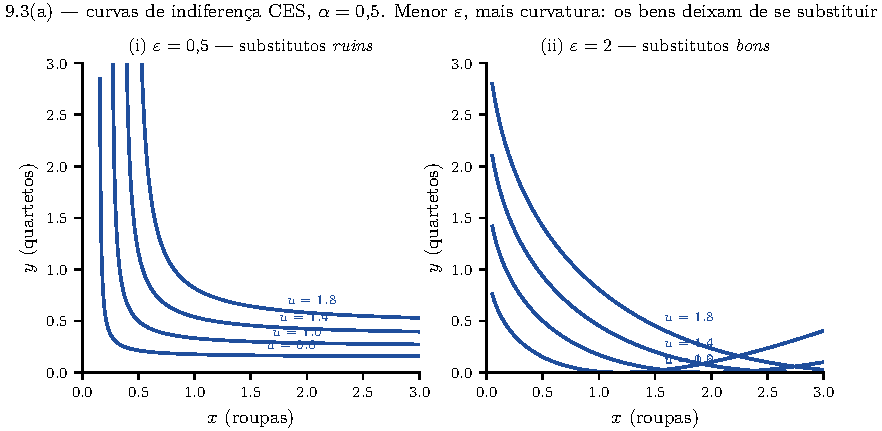
\includegraphics[width=\linewidth]{fig/fig_k9_3_ces.pdf}\\[3pt]
\captionof{figure}{Problem 9.3(a). CES indifference curves.}
\label{fig:ces}
\end{center}

\item The household maximises $u(x,y)$ subject to $p_xx+p_yy=w$. The stated result is the
standard CES demand system; the essential content is that $p$ is the \textbf{exact price index}
for this utility function, meaning $u=w/p$ at the optimum. The two demands say the household
spends its real income $w/p$ on the two goods with expenditure shares that respond to relative
prices with elasticity $\epsilon$. Setting $\epsilon=1$ collapses them to the Cobb-Douglas case
$p_xx=\alpha w$, $p_yy=(1-\alpha)w$, in which shares are constant --- a useful check.

\item Each firm's problem is linear:
\[
\max_{L_x}\ p_xA_xL_x-wL_x=(p_xA_x-w)L_x,
\qquad
\max_{L_y}\ (p_yA_y-w)L_y .
\]
This is the same structure as the investment firm's problem (9.1.2): a linear objective has no
interior optimum. If the coefficient is positive the firm hires infinite labour; if negative it
hires none. A positive, finite quantity requires the coefficient to be exactly zero:
\[
\boxed{\ \frac{p_x}{w}=\frac{1}{A_x},\qquad \frac{p_y}{w}=\frac{1}{A_y}\ }.
\]
Price equals unit labour cost, and profits are zero.

\item Dividing the two:
\[
\boxed{\ \frac{p_y}{p_x}=\frac{A_x}{A_y}\ }.
\]
The relative price of a good is the \emph{inverse} of its relative productivity. Note what is
absent: preferences. Demand has no effect whatever on relative prices here, because both
technologies are linear --- supply curves are horizontal.

\item $A_x$ rising with $A_y$ constant means productivity grows in manufacturing but not in the
performing arts. \textbf{This is highly plausible}, and it is Baumol's original observation: a
loom is many times more productive than it was in 1800, while a Schubert quartet still requires
four musicians and forty minutes, exactly as it did then. Some activities have essentially no
scope for labour-saving technical change because the labour \emph{is} the product.

By (d), the relative price of performances rises \textbf{one for one} with $A_x$. The reason is
the labour market, not the concert hall: as manufacturing becomes more productive it can pay
more, and quartets must match that wage to keep their players, without any offsetting
productivity gain to absorb it. Live performance therefore gets steadily more expensive relative
to goods --- the \textbf{cost disease}. The same logic applies to education, health care,
haircuts and legal services, which is why their relative prices have risen for a century.

\item From (b), taking the ratio of the two demands:
\[
\frac{y}{x}=\frac{(1-\alpha)(p_y/p)^{-\epsilon}}{\alpha(p_x/p)^{-\epsilon}}
=\frac{1-\alpha}{\alpha}\left(\frac{p_y}{p_x}\right)^{-\epsilon}
\;\Longrightarrow\;
\boxed{\ \frac{y}{x}=\frac{1-\alpha}{\alpha}\left(\frac{A_x}{A_y}\right)^{-\epsilon}\ }.
\]
Performances always fall relative to clothes as $A_x$ grows, at a rate governed by $\epsilon$.

\item Labour used is $L_x=x/A_x$ and $L_y=y/A_y$, so
\[
\frac{L_y}{L_x}=\frac{y/A_y}{x/A_x}=\frac{y}{x}\cdot\frac{A_x}{A_y}
=\frac{1-\alpha}{\alpha}\left(\frac{A_x}{A_y}\right)^{-\epsilon}\frac{A_x}{A_y}
\;\Longrightarrow\;
\boxed{\ \frac{L_y}{L_x}=\frac{1-\alpha}{\alpha}\left(\frac{A_x}{A_y}\right)^{1-\epsilon}\ }.
\]
The exponent has flipped sign relative to (f), and everything now turns on whether
$\epsilon$ is above or below one.

\item Write $R\equiv L_y/L_x$ from part (g). Since $L_x+L_y=1$,
\[
L_y=\frac{R}{1+R},\qquad y=A_yL_y=\frac{A_yR}{1+R}.
\]
$A_y$ is constant, so the quantity of performances moves exactly as $R$ does, and
$R\propto (A_x/A_y)^{1-\epsilon}$. Three regimes:
\begin{center}
\begin{tabular}{lll}
\toprule
\textbf{Case} & \textbf{Labour share in quartets} & \textbf{Performances $y$} \\
\midrule
$\epsilon<1$ (poor substitutes) & rises toward 1 & \textbf{rises} toward $A_y$ \\
$\epsilon=1$ (Cobb-Douglas) & constant & \textbf{constant} \\
$\epsilon>1$ (good substitutes) & falls toward 0 & \textbf{falls} toward 0 \\
\bottomrule
\end{tabular}
\end{center}

\emph{Reading.} Two forces run against each other. Quartets get relatively more expensive,
which pushes consumers away; but if the goods are poor substitutes, consumers refuse to give
them up and must devote an ever-larger \emph{share of spending}, and therefore of labour, to
buying them. When $\epsilon<1$ the second force wins and the stagnant sector absorbs the whole
economy --- the strong form of the cost disease, and the reason health and education keep rising
as a share of GDP even as their relative price rises. When $\epsilon>1$ consumers substitute
away and the sector withers, which is closer to the story of live theatre displaced by recorded
media. The empirical relevance of the cost disease is thus an argument about $\epsilon$.
\end{enumerate}

\begin{tcolorbox}[trapbox]
Do not read (f) and (h) as contradictory. The \emph{ratio} $y/x$ always falls --- part (f) has
$-\epsilon<0$ in the exponent for any $\epsilon>0$. What can rise is the \emph{level} of $y$,
because $x$ is growing so fast that $y$ can rise while still falling relative to it. The two
statements answer different questions, and the exercise is built to make you notice.
\end{tcolorbox}
\end{tcolorbox}

%---- Topic: Steady State, Dynamics and Anticipation ----
\subsection{Steady State, Dynamics and Anticipation}

%------- 9.6 -------
% Topic: Steady State, Dynamics and Anticipation
% Keywords: capital income tax, after-tax Euler equation, steady state, tax incidence, Judd-Chamley
\begin{tcolorbox}[evenbox,title={Problem 9.6 \quad Capital Income Taxes}]
\begin{tcolorbox}[questionbox]
An economy has production function $Y=K^\alpha L^{1-\alpha}$ and two types of households.
Workers supply $L$ units of labour inelastically and consume all their income:
$c_t=w_tL+T_t$, where $T_t$ is a government transfer. Capitalists have preferences
$\sum_{t=0}^{\infty}\beta^tu(c_t)$, do not work, and face the budget constraint
\[
K_{t+1}=-c_t+\Big[1+(1-\tau)\big(r^K_t-\delta\big)\Big]K_t .
\]
The government taxes the rental on capital, net of depreciation, at rate $\tau$, and taxes
interest income in the same way, so that (9.1.11) holds.\\[3pt]
(a) Set up the capitalist household's maximisation problem.\\
(b) From the first-order conditions, find an after-tax version of the Euler equation.\\
(c) If in the long run the economy reaches a steady state with constant capitalist
consumption, what are the pre-tax and after-tax interest rates?\\
(d) In steady state, what is the rental rate of capital? How does it depend on $\tau$?\\
(e) In steady state, what is the capital stock?\\
(f) How much revenue does the government collect in steady state?\\
(g) What is the level of wages in steady state?\\
(h) Suppose the government uses all the revenue to finance transfers to workers. What level of
consumption do workers attain in steady state? How does it depend on $\tau$? Explain.
\end{tcolorbox}

\textbf{Solution:}

\begin{enumerate}
\item Writing $R_t\equiv 1+(1-\tau)\big(r^K_t-\delta\big)$ for the after-tax gross return,
\[
\max_{\{c_t,K_{t+1}\}}\ \sum_{t=0}^{\infty}\beta^t u(c_t)
\qquad\text{s.t.}\qquad
K_{t+1}=R_tK_t-c_t,\quad K_0\ \text{given},
\]
plus a no-Ponzi condition. The capitalist takes $r^K_t$ as given even though it depends on the
aggregate capital stock --- the standard atomistic assumption.

\item Substituting $c_t=R_tK_t-K_{t+1}$ into the objective and differentiating with respect to
$K_{t+1}$:
\[
-u'(c_t)+\beta u'(c_{t+1})R_{t+1}=0
\;\Longrightarrow\;
\boxed{\ u'(c_t)=\beta\Big[1+(1-\tau)\big(r^K_{t+1}-\delta\big)\Big]u'(c_{t+1})\ }.
\]
This is (9.3.8) with the gross interest factor replaced by its after-tax counterpart. The
household discounts using the return it actually receives, not the one the firm pays.

\item In a steady state $c_{t+1}=c_t$, so $u'(c_t)=u'(c_{t+1})$ and the Euler equation collapses
to $1=\beta\big[1+(1-\tau)(r^K-\delta)\big]$. Writing $\rho\equiv\frac{1}{\beta}-1$ for the rate
of time preference:
\[
\boxed{\ r^{\text{after}}=(1-\tau)\big(r^K-\delta\big)=\rho=\frac{1}{\beta}-1\ },
\qquad
\boxed{\ r^{\text{pre}}=r^K-\delta=\frac{\rho}{1-\tau}\ }.
\]

\emph{Reading, and it is the central result of the problem.} The \textbf{after-tax} rate is
pinned to $\rho$ by preferences alone --- the tax cannot touch it. Everything therefore adjusts
so that the \textbf{pre-tax} rate rises to $\rho/(1-\tau)$. The capitalists do not absorb the
tax; the required return before tax simply climbs until they are made whole again. Whoever ends
up paying, it is not them.

\item From (c), $r^K=\delta+\dfrac{\rho}{1-\tau}$, which is \textbf{increasing in $\tau$} and
rises without bound as $\tau\to1$.

\item Setting $F_K=r^K$ with labour fixed at $L$:
\[
\alpha\left(\frac{K}{L}\right)^{\alpha-1}=\delta+\frac{\rho}{1-\tau}
\;\Longrightarrow\;
\boxed{\ K\stst=L\left[\frac{\alpha}{\ \delta+\frac{\rho}{1-\tau}\ }\right]^{\frac{1}{1-\alpha}}\ },
\]
which is \textbf{decreasing in $\tau$}. Higher required pre-tax return means less capital.

\item Revenue is the tax rate times the taxed base:
\[
\boxed{\ T=\tau\big(r^K-\delta\big)K\stst=\tau\,\frac{\rho}{1-\tau}\,K\stst\ }.
\]
Note that this is not monotone in $\tau$: the rate rises but the base shrinks --- a Laffer
shape. As $\tau\to1$, $K\stst\to0$ fast enough that revenue goes to zero.

\item $w=F_L=(1-\alpha)\left(\dfrac{K\stst}{L}\right)^{\alpha}$, which \textbf{falls with
$\tau$} because $K\stst$ does. This is the transmission channel: the tax on capital arrives at
workers as a lower wage.

\item Workers consume wages plus the transfer:
\[
c^{w}=\underbrace{(1-\alpha)(K\stst)^{\alpha}L^{1-\alpha}}_{wL,\ \text{falling in }\tau}
+\underbrace{\tau\frac{\rho}{1-\tau}K\stst}_{T,\ \text{hump-shaped in }\tau} .
\]
Two forces, opposite signs. Evaluate the trade-off at $\tau=0$:
\begin{align*}
\text{marginal revenue gain}\quad
&\dd{T}{\tau}\bigg|_{0}=\rho K\stst,\\[4pt]
\text{marginal wage loss}\quad
&-\dd{(wL)}{\tau}\bigg|_{0}=\alpha\,\frac{\rho}{r^K}\,Y
\qquad\text{(from }\dd{\ln Y}{\tau}=-\tfrac{\alpha}{1-\alpha}\tfrac{\rho}{r^K}\text{).}
\end{align*}
But the firm's first-order condition says $r^K=F_K=\alpha Y/K\stst$, hence
$\alpha Y/r^K=K\stst$ and the two expressions are \textbf{identical}:
\[
\boxed{\ \dd{c^{w}}{\tau}\bigg|_{\tau=0}=\rho K\stst-\rho K\stst=0\ }
\]

\begin{tcolorbox}[databox]
The code confirms it to machine precision: with $\alpha=0{,}4$, $\beta=0{,}95$, $\delta=0{,}08$,
$L=1$, the numerical derivative at $\tau=0$ is $-1{,}1\times10^{-7}$, and the second derivative
is $-0{,}219<0$, so $\tau=0$ is a \textbf{maximum}.
\begin{center}
\small
\begin{tabular}{cccccc}
\toprule
$\tau$ & $r^K$ & $K\stst$ & $Y$ & $wL$ & $c^{w}$ \\
\midrule
$0{,}00$ & $0{,}1326$ & $6{,}295$ & $2{,}087$ & $1{,}2524$ & $\mathbf{1{,}2524}$ \\
$0{,}05$ & $0{,}1354$ & $6{,}082$ & $2{,}059$ & $1{,}2353$ & $1{,}2522$ \\
$0{,}10$ & $0{,}1385$ & $5{,}859$ & $2{,}028$ & $1{,}2169$ & $1{,}2512$ \\
$0{,}20$ & $0{,}1458$ & $5{,}377$ & $1{,}960$ & $1{,}1759$ & $1{,}2467$ \\
$0{,}40$ & $0{,}1677$ & $4{,}257$ & $1{,}785$ & $1{,}0710$ & $1{,}2204$ \\
$0{,}60$ & $0{,}2116$ & $2{,}891$ & $1{,}529$ & $0{,}9174$ & $1{,}1456$ \\
\bottomrule
\end{tabular}
\end{center}
\end{tcolorbox}

\textbf{Answer.} Workers' steady-state consumption is \textbf{maximised at $\tau=0$} and falls
for every positive tax rate, \emph{even though every cent of revenue is handed to them}.

\smallskip
\emph{Reading.} At the margin, the first unit of revenue raised costs workers exactly one unit
of wages --- the two effects cancel because the rental rate the government taxes is precisely
the marginal product of the capital that the tax destroys. Beyond that first unit, the base
keeps shrinking and the losses compound, so the net effect turns negative. A tax whose whole
proceeds are given to workers still leaves them worse off. This is a miniature of the
Judd--Chamley result that the optimal long-run capital income tax is zero, and it is a warning
that the \emph{statutory} incidence of a tax says nothing about who bears it.
\end{enumerate}
\end{tcolorbox}

%------- 9.9 -------
% Topic: Steady State, Dynamics and Anticipation
% Keywords: phase diagram, saddle path, anticipated shock, endowment, wealth effect
\begin{tcolorbox}[oddbox,title={Problem 9.9 \quad An Oil-Producing Economy}]
\begin{tcolorbox}[questionbox]
Suppose the production function is $F(K,L)=K^\alpha L^{1-\alpha}+e$. GDP is the sum of regular
output, produced with capital and labour, and oil extraction $e$, which is exogenous. The
representative household has preferences $\sum_{t=0}^{\infty}\beta^t\log(c_t)$ and supplies
$L=1$ units of labour inelastically. Capital depreciates at rate $\delta$.\\[3pt]
(a) On the same graph, draw two phase diagrams, one for $e=0$ and one for $e=\bar e>0$, and
label the steady state in each case.\\
(b) Suppose the economy starts at $t=0$ at the $\bar e$ steady state but everyone suddenly
realises oil will run out at time $T$, so that $e_t=\bar e$ for $t<T$ and $e_t=0$ for
$t\ge T$. Using the phase diagrams, plot the evolution of $K_t$ and $c_t$ from $t=0$ to $T$
and from $T$ onwards. Describe in words why consumption and investment evolve the way they do,
and what happens to wages and the interest rate.
\end{tcolorbox}

\textbf{Solution:}

\begin{enumerate}
\item Build the two loci from (9.3.14) and (9.3.15), with $L=1$ and $\sigma=1$ (log utility).

\textbf{The $\Delta c=0$ locus.} Setting $c_{t+1}=c_t$ in (9.3.14) gives
$\beta\big(1+F_K(K,1)-\delta\big)=1$, that is
\[
\alpha K^{\alpha-1}-\delta=\frac{1}{\beta}-1 .
\]
The oil term $e$ is \textbf{additive} and therefore vanishes on differentiation:
$F_K=\alpha K^{\alpha-1}$ whether or not there is oil. So the vertical line sits at
\[
K\stst=\left[\frac{\alpha}{\frac{1}{\beta}-1+\delta}\right]^{\frac{1}{1-\alpha}}
\qquad\textbf{--- identical in the two economies.}
\]

\textbf{The $\Delta K=0$ locus.} Setting $K_{t+1}=K_t$ in (9.3.15):
\[
c=F(K,1)-\delta K=K^{\alpha}+e-\delta K,
\]
which is the same concave curve \textbf{shifted up by exactly $e$}.

\smallskip
So the two diagrams share a vertical line and differ by a parallel vertical shift of the curve.
The two steady states have the \textbf{same capital stock} and consumption differing by exactly
$\bar e$: the oil is consumed, not invested. See panel (i) of Figure~\ref{fig:fase}.

\begin{center}
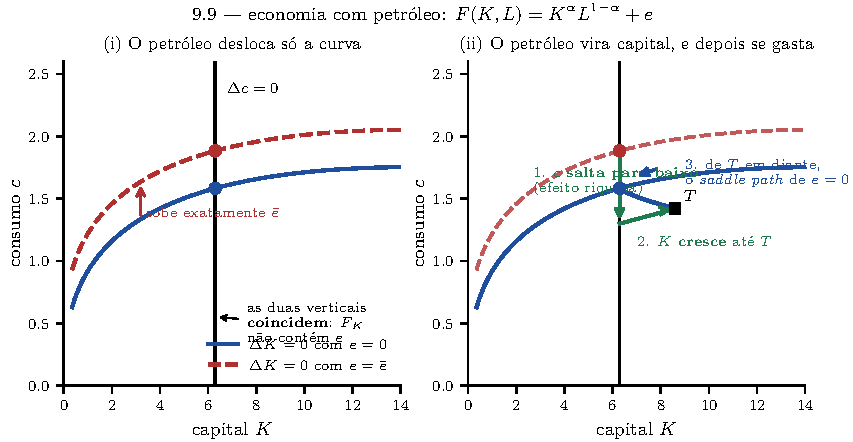
\includegraphics[width=\linewidth]{fig/fig_k9_9_fase.pdf}\\[3pt]
\captionof{figure}{Problem 9.9. Left: the two phase diagrams. Right: the transition when oil runs out at
$T$. Drawn with $\alpha=0{,}4$, $\beta=0{,}95$, $\delta=0{,}08$, $\bar e=0{,}30$.}
\label{fig:fase}
\end{center}

\item Three phases, shown in panel (ii).

\textbf{At $t=0$: consumption jumps down.} The news makes the household permanently poorer in
present-value terms --- a stream of $\bar e$ that was expected forever now stops at $T$. With
$K_0=K\stst$ fixed (capital is a state variable and cannot jump), the only variable free to
respond is consumption, and it falls immediately. The size of the jump is not free: it is pinned
down by the requirement in the next paragraph.

\textbf{From $0$ to $T$: capital accumulates.} Consumption is now \emph{below} the
$\Delta K=0$ curve for the $\bar e$ economy, so investment exceeds depreciation and $K$ rises.
Meanwhile $K>K\stst$ makes $F_K$ fall below $\rho+\delta$, so by (9.3.14) consumption
\emph{declines} gradually along the way. The economy is converting its oil windfall into capital
while it still has it.

\textbf{At $T$ and after.} The $\Delta K=0$ curve drops by $\bar e$. The point
$(K_T,c_T)$, which was below the old curve, is now \emph{above} the new one, so capital begins to
fall. The economy must arrive at $T$ exactly on the $e=0$ saddle path --- and it is this
requirement, working backwards, that determined the size of the jump at $t=0$. From $T$ onward
it slides down that saddle path, running the capital stock back down to $K\stst$ while
consumption falls to $c\stst=(K\stst)^{\alpha}-\delta K\stst$.

\smallskip
\textbf{Prices.} $w=(1-\alpha)K^{\alpha}$ and $r=\alpha K^{\alpha-1}-\delta$ depend only on $K$.
So during $[0,T)$ the wage \textbf{rises} and the interest rate \textbf{falls} as capital is
accumulated; after $T$ both retrace as capital is run down. The oil boom shows up in the labour
market as a temporary wage premium that vanishes with the resource.

\smallskip
\emph{Reading.} This is the case for a sovereign wealth fund, derived rather than asserted. A
country that knows its resource is finite should not consume the flow; it should convert it into
a stock of productive capital that can be drawn down when the resource is gone. The model says
consumption \emph{never} rises during the boom --- it jumps down at the announcement and
declines throughout --- which is precisely the discipline that resource-rich countries find
hard, and the failure of which is one component of the resource curse.
\end{enumerate}
\end{tcolorbox}

%------- 9.10 -------
% Topic: Steady State, Dynamics and Anticipation
% Keywords: model building, endowment stream, capital as livestock, anticipation, interest rate determination
\begin{tcolorbox}[evenbox,title={Problem 9.10 \quad Wizards and Cows}]
\begin{tcolorbox}[questionbox]
The Calevingians have two economic activities: gathering fruit and raising cows. Wild fruit
grows in the West; they cannot cultivate it and simply pick what is ripe, spread evenly through
the year. Warm years yield plentiful fruit, colder years less. They trust their chief wizard,
who gives a fruit forecast with a horizon of a few years. Cows graze in the East; each family
owns a plot and keeps its own cows. Cows are raised for meat only. A main decision is how many
cows to slaughter each year and how many (including calves) to keep fattening from one year to
the next; the more cows kept on a plot, the less grass each has.\\[3pt]
(a) Write down mathematically the economic decision problem faced by a Calevingian household.
Explain the meaning of each equation.\\
(b) Derive first-order conditions.\\
(c) Suppose the wizard announces that the next few years will be cold and yield less fruit. How
do households react?\\
(d) The Calevingians have well-enforced contracts, sales, loans and interest rates: one can
borrow to buy cows, or sell cows and lend the proceeds. What happens to interest rates when the
wizard announces the cold weather?
\end{tcolorbox}

\textbf{Solution:}

\begin{enumerate}
\item The problem is the neoclassical growth model in costume. Read the story into the symbols:
\begin{center}
\begin{tabular}{@{}ll@{}}
\toprule
\textbf{In the story} & \textbf{In the model} \\
\midrule
Fruit picked in year $t$ & exogenous endowment $y_t$, known in advance \\
The herd kept at the start of $t$ & capital stock $K_t$ \\
Calves born, net of crowding & production $f(K_t)$, with $f'>0$, $f''<0$ \\
Cows that die of natural causes & depreciation $\delta K_t$ \\
Cows slaughtered for meat & consumption out of the herd \\
The wizard's forecast & perfect foresight over $\{y_t\}$ \\
\bottomrule
\end{tabular}
\end{center}
The household solves
\[
\max_{\{c_t,K_{t+1}\}}\ \sum_{t=0}^{\infty}\beta^t u(c_t)
\qquad\text{s.t.}\qquad
c_t+K_{t+1}=y_t+f(K_t)+(1-\delta)K_t,\quad K_0\ \text{given}.
\]
The constraint is a resource identity: everything eaten this year plus the herd carried into
next year must equal the fruit picked, plus the calves born, plus the cows that survived.
Diminishing returns, $f''<0$, is the grass constraint --- the model's entire economic content on
the production side.

\item Substituting the constraint and differentiating with respect to $K_{t+1}$:
\[
\boxed{\ u'(c_t)=\beta\Big[1+f'(K_{t+1})-\delta\Big]u'(c_{t+1})\ },
\]
the Euler equation (9.3.13). In the story: the meat given up by \emph{not} slaughtering one more
cow today must be worth, at the margin, the extra cows it produces plus itself, valued at
tomorrow's marginal utility and discounted.

\item Lower future fruit is a \textbf{negative wealth shock}. Since $y_t$ enters the resource
constraint additively, exactly like the oil in Problem 9.9, the household is permanently poorer
and consumption \textbf{falls immediately} --- before a single cold day arrives. Slaughtering
falls, so the herd is \textbf{built up} in anticipation of the lean years, and then drawn down
while they last. The Calevingians save by keeping cows because keeping cows is the only way to
save.

\smallskip
Note the mechanism has nothing to do with the weather affecting cows: grass grows equally well in
cold and warm years, by assumption. The response is entirely intertemporal substitution driven by
foresight, and it would not exist without the wizard.

\item Interest rates \textbf{fall}. Two ways to see it, and they are the same fact.

\textbf{Through the technology.} Arbitrage (9.3.11) ties the interest rate to the return on the
only asset in the economy:
\[
1+r_{t+1}=1+f'(K_{t+1})-\delta .
\]
The herd grows, so grass per cow falls, so $f'(K_{t+1})$ falls, so $r$ falls.

\textbf{Through the market.} Everyone wants to save at once, and nobody wants to borrow. The
supply of loans jumps and demand does not. The price of future goods in terms of present goods
rises, which is exactly what a lower interest rate means.

\smallskip
\emph{Reading.} This is the classic result that news of future scarcity depresses the real
interest rate today --- a precautionary-saving story without any uncertainty in it, since the
wizard is never wrong. Interest rates in this economy carry information about what everybody
expects, which is why they are watched.
\end{enumerate}
\end{tcolorbox}

%------- 9.11 -------
% Topic: Steady State, Dynamics and Anticipation
% Keywords: steady state, Cobb-Douglas, patience, investment rate, Golden Rule comparison
\begin{tcolorbox}[oddbox,title={Problem 9.11 \quad Patience and Investment}]
\begin{tcolorbox}[questionbox]
Suppose the production function is $F(K,L)=K^{\alpha}L^{1-\alpha}$ and labour supply is exogenous
and equal to $L=1$. The representative household's preferences are
$\sum_{t=0}^{\infty}\beta^t\frac{c_t^{1-\sigma}}{1-\sigma}$ and the depreciation rate is
$\delta$.\\[3pt]
(a) Use equation (9.3.17) to find an expression for the level of capital this economy will have
in the steady state.\\
(b) Find an expression for the level of GDP in the steady state. How does it depend on
$\beta$?\\
(c) Find an expression for the steady-state investment-to-GDP ratio. Explain.
\end{tcolorbox}

\textbf{Solution:}

Throughout write $\rho\equiv\frac{1}{\beta}-1$ for the rate of time preference.

\begin{enumerate}
\item Equation (9.3.17) with $F_K=\alpha K^{\alpha-1}$ and $L=1$:
\[
\alpha (K\stst)^{\alpha-1}-\delta=\frac{1}{\beta}-1
\;\Longrightarrow\;
(K\stst)^{\alpha-1}=\frac{\rho+\delta}{\alpha}
\;\Longrightarrow\;
\boxed{\ K\stst=\left(\frac{\alpha}{\rho+\delta}\right)^{\frac{1}{1-\alpha}}\ }.
\]

\textbf{Note what is missing: $\sigma$.} The intertemporal elasticity governs how \emph{fast}
the economy travels but not \emph{where} it ends up. Only $\alpha$, $\beta$ and $\delta$ appear.

\item $Y\stst=(K\stst)^{\alpha}$, so
\[
\boxed{\ Y\stst=\left(\frac{\alpha}{\rho+\delta}\right)^{\frac{\alpha}{1-\alpha}}\ }.
\]
A higher $\beta$ means a lower $\rho$, hence a smaller denominator and a \textbf{higher}
$Y\stst$: patient countries end up richer. The elasticity of $Y\stst$ with respect to
$(\rho+\delta)$ is $-\frac{\alpha}{1-\alpha}$, which with $\alpha=1/3$ is $-1/2$ --- the same
elasticity that governs the response of steady-state output to the saving rate in the Solow
model of Chapter 5, and it is small for the same reason.

\item In steady state gross investment just replaces depreciation, $I=\delta K\stst$, so
\[
\frac{I}{Y}=\frac{\delta K\stst}{(K\stst)^{\alpha}}=\delta (K\stst)^{1-\alpha}
=\delta\cdot\frac{\alpha}{\rho+\delta}
\;\Longrightarrow\;
\boxed{\ \frac{I}{Y}=\frac{\alpha\,\delta}{\rho+\delta}\ }.
\]

\emph{Reading, and it is the punchline of the chapter.} This is the saving rate that an
exogenous-saving Solow economy would need in order to land on the same steady state. Compare it
with the \textbf{Golden Rule} rate, which for Cobb-Douglas is $s_{gr}=\alpha$:
\[
\frac{I}{Y}=\alpha\cdot\underbrace{\frac{\delta}{\rho+\delta}}_{<\,1\ \text{whenever}\ \rho>0}
\;<\;\alpha=s_{gr}.
\]
The economy \textbf{always} invests less than the Golden Rule prescribes, and the gap is
\emph{exactly} the factor $\frac{\delta}{\rho+\delta}$ --- a clean measure of how much
impatience costs in terms of steady-state capital. As $\beta\to1$ we have $\rho\to0$ and the
ratio goes to $\alpha$: an infinitely patient economy chooses the Golden Rule after all.

\begin{tcolorbox}[databox]
With $\alpha=0{,}4$, $\beta=0{,}95$, $\delta=0{,}08$: $\rho=0{,}05263$,
$K\stst=6{,}2954$, $Y\stst=2{,}0874$, and $I/Y=0{,}2413$ against a Golden Rule rate of
$0{,}40$. The Golden Rule capital stock is
$K_{gr}=(\alpha/\delta)^{1/(1-\alpha)}=14{,}62$, more than twice $K\stst$. \checkmark
\end{tcolorbox}
\end{enumerate}
\end{tcolorbox}

%------- 9.12 -------
% Topic: Steady State, Dynamics and Anticipation
% Keywords: shooting method, saddle path, consumption-equivalent welfare, transition dynamics, Solow comparison
\begin{tcolorbox}[evenbox,title={Problem 9.12 \quad Optimal vs Fixed Savings Rates}]
\begin{tcolorbox}[questionbox]
Suppose the economy is as in Exercise 9.11, with $\alpha=0.4$, $\beta=0.95$, $\delta=0.08$ and
$\sigma=2$. The economy starts with $K_0=2$. Compare how it behaves under a fixed investment
rate and under an optimally chosen one.\\[3pt]
(a) First suppose the investment rate is exogenous and constant, equal to the steady-state
investment-to-GDP ratio found in Exercise 9.11. Compute GDP, consumption, investment and the
capital stock for the first 150 years.\\
(b) Now suppose consumption and investment are chosen in accordance with (9.3.13). Find the
level of initial consumption consistent with (9.3.15)--(9.3.13) and convergence to a steady
state. Compute the same four series for 150 years.\\
(c) Plot the consumption paths of the two economies on the same graph.\\
(d) Substitute the computed consumption paths into the utility function to compute the utility
obtained in each economy over the first 150 years.\\
(e) By what fraction would consumption in the optimal-savings economy have to be reduced for the
household to obtain the same utility as in the exogenous-savings economy?
\end{tcolorbox}

\textbf{Solution:}

\begin{enumerate}
\item From 9.11(c), $s=\dfrac{\alpha\delta}{\rho+\delta}=0{,}241270$. Iterate
\[
Y_t=K_t^{\alpha},\quad I_t=sY_t,\quad c_t=(1-s)Y_t,\quad
K_{t+1}=(1-\delta)K_t+I_t,\qquad K_0=2 .
\]

\item The optimal path must satisfy the two difference equations
\[
K_{t+1}=(1-\delta)K_t+K_t^{\alpha}-c_t,
\qquad
\frac{c_{t+1}}{c_t}=\big[\beta\big(1+\alpha K_{t+1}^{\alpha-1}-\delta\big)\big]^{1/\sigma},
\]
and converge. Only one $c_0$ does: the one on the saddle path. Solve by \textbf{shooting} ---
iterate forward from a candidate $c_0$ and bisect on whether the path diverges toward zero
capital (if $c_0$ is too high) or toward zero consumption (if too low). The code gives
\[
\boxed{\ c_0=0{,}9206271904\ }
\]
against the fixed-rate economy's $c_0=(1-s)\cdot2^{0{,}4}=1{,}00115$.

\item See Figure~\ref{fig:c912}.

\begin{center}
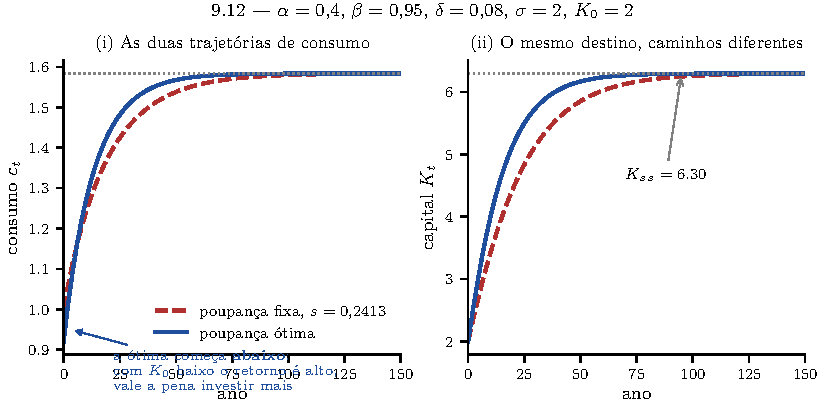
\includegraphics[width=\linewidth]{fig/fig_k9_12_consumo.pdf}\\[3pt]
\captionof{figure}{Problem 9.12(c). Consumption and capital under a fixed and an optimal investment rate,
from $K_0=2$.}
\label{fig:c912}
\end{center}

\begin{tcolorbox}[databox]
\small
\begin{center}
\begin{tabular}{rrrrr}
\toprule
$t$ & $K$ fixed & $K$ optimal & $c$ fixed & $c$ optimal \\
\midrule
$0$ & $2{,}000$ & $2{,}000$ & $\mathbf{1{,}0012}$ & $\mathbf{0{,}9206}$ \\
$5$ & $2{,}760$ & $3{,}117$ & $1{,}1389$ & $1{,}1297$ \\
$10$ & $3{,}426$ & $4{,}005$ & $1{,}2417$ & $\mathbf{1{,}2719}$ \\
$25$ & $4{,}832$ & $5{,}496$ & $1{,}4248$ & $1{,}4818$ \\
$50$ & $5{,}851$ & $6{,}167$ & $1{,}5381$ & $1{,}5678$ \\
$149$ & $6{,}292$ & $6{,}295$ & $1{,}5834$ & $1{,}5838$ \\
\midrule
ss & $6{,}2954$ & $6{,}2954$ & $1{,}5838$ & $1{,}5838$ \\
\bottomrule
\end{tabular}
\end{center}
\end{tcolorbox}

\textbf{The shape of the answer.} The optimal economy consumes \emph{less} than the fixed-rate
economy at first and \emph{more} later, crossing over around year 8. The reason is visible in
9.11: at $K_0=2$, far below $K\stst=6{,}30$, the marginal product of capital is very high, so the
return to investing is unusually good and the household takes it. A fixed rate cannot respond to
that --- it invests the same fraction whether capital is scarce or abundant.

\item With $\sigma=2$, $u(c)=\frac{c^{-1}}{-1}=-\frac{1}{c}$. Summing
$\sum_{t=0}^{149}\beta^tu(c_t)$:
\[
U^{\text{fixed}}=-15{,}799881,
\qquad
U^{\text{optimal}}=-15{,}743595 .
\]
Both are negative, as CRRA with $\sigma>1$ requires; the optimal path is closer to zero, hence
better. \checkmark

\item Scaling all optimal consumption by $\lambda$ multiplies utility by $\lambda^{1-\sigma}$,
so $\lambda$ solves $\lambda^{1-\sigma}U^{\text{optimal}}=U^{\text{fixed}}$:
\[
\lambda=\left(\frac{U^{\text{fixed}}}{U^{\text{optimal}}}\right)^{\frac{1}{1-\sigma}}
=\left(\frac{-15{,}799881}{-15{,}743595}\right)^{-1}
=\boxed{0{,}996438}.
\]
Consumption in the optimal economy would have to be cut by
\[
1-\lambda=\mathbf{0{,}356\%}
\]
for the household to be indifferent between the two.

\smallskip
\emph{Reading --- and the surprise is how small this is.} Optimising the entire savings path,
period by period, for 150 years, is worth about a third of one percent of consumption. The reason
is structural, not numerical: the fixed rate used in part (a) is not an arbitrary number, it is
\emph{the correct steady-state rate}, so the two economies have the same destination and the same
long-run consumption. All that differs is the shape of the transition, and consumption smoothing
makes utility quite flat with respect to that shape.

\smallskip
This is a specific instance of a general finding in this literature, and it cuts both ways. It
justifies the Solow model as a workhorse --- assuming a constant saving rate costs almost nothing
in welfare terms when the rate is right. It also warns that welfare comparisons of transition
paths are a weak instrument: if 150 years of visibly different investment behaviour is worth
$0{,}36\%$, then a model that gets the steady state wrong matters far more than one that gets the
dynamics wrong.
\end{enumerate}
\end{tcolorbox}

%======================================================================
\section*{Companion code}
\addcontentsline{toc}{section}{Companion code}
%======================================================================

Every numerical result above is reproduced by \texttt{Resolucao/kurlat\_ch09\_codigo/}. Each
script checks its analytical formulas against an independent numerical computation and aborts on
any mismatch.

\begin{center}
\begin{tabular}{@{}lp{10.2cm}@{}}
\toprule
\textbf{File} & \textbf{What it does} \\
\midrule
\texttt{ch09\_numerico.py} & Problem 9.11: verifies (9.3.17) and $I/Y=\alpha\delta/(\rho+\delta)$
against $\delta (K\stst)^{1-\alpha}$, and $K\stst<K_{gr}$. Problem 9.6: the table of steady states,
plus a finite-difference check that $\dd{c^w}{\tau}=0$ at $\tau=0$ and that the second derivative
is negative. Problem 9.12: the shooting solution for $c_0$, both 150-year paths, and $\lambda$.
Problem 9.13: the two labour allocations, the GDP gap, and the wage and rental changes. \\
\texttt{ch09\_figuras.py} & The three figures. \\
\texttt{estilo\_mpl.py} & \texttt{pgf} backend, so figure text is typeset by \texttt{pdflatex}
with \texttt{lmodern} and \texttt{cmap} and the PDF stays fully copyable. \\
\bottomrule
\end{tabular}
\end{center}

\end{document}
